\section{Non-Clairvoyant Algorithm}

Auction methods have been effectively used for assignment problems in dynamic multi-agent environments \cite{Mehta05,Lagoudakis04}. With these methods, each worker (agent) places a bid on each task and task assignment is achieved by a process similar to winner determination in auctions. One key advantage of auction-based assignment is that each worker can compute its own bid independent of other workers. Therefore, a great portion of the computation can be decentralized which in turn helps to whole process to scale faster. In this section, we introduce a generic framework for auction-based task assignment in spatial crowdsourcing and introduce a variety of bidding rules based on different heuristics.\\

Our auction-based framework considers the workers as bidders and tasks as goods, and operates as follows. Upon arrival of each task, it performs one round of bidding. During each round of bidding, all workers bid on the task. Depending on the bidding rule, the worker with the overall highest/lowest bid wins and is assigned to that particular task. Upon assignment of a new task, each worker updates its path based on the task(s) that it has been assigned to and moves along that path.\\

The main advantage of this auction-based mechanism is its simplicity and, as mentioned earlier, the fact that it allows for a decentralized implementation for each worker. Each worker only needs to know its own location, the location of the new task but not the location of any other worker. In each round, each worker computes its single bid locally and in parallel with the other workers and reports the bid to the \textit{SC server}. The server, which plays the role of a central auctioneer, chooses the winning worker and assigns the task to it. It is worth to mention the low cost of communication in our framework; each worker submits only one number to the server in each round of bidding. In addition, workers do not have to share their own location with any other entity (including the server) which preserves their privacy.\\

\begin{algorithm}
\caption{OnlineTASC($W, t$)}
\label{algo:OnlineTASC}
\begin{algorithmic}[1]
\REQUIRE $W$ is the set of currently available workers and $t$ is a task the has just released
\ENSURE Either $w \in W$ as the worker task $t$ should be assigned to or \emph{null} if no worker is selected
\STATE $w_{selected} = $ \emph{null}
\STATE $Bids = \emptyset$
\FOR{$w \in W$}
	\STATE $bid = w$.ComputeBid$(t)$
	\STATE $Bids \leftarrow \left\langle w, bid \right\rangle$
\ENDFOR
\STATE $w_{selected} = $ SelectBestBid$(Bids)$
\RETURN $w_{selected}$
\end{algorithmic}
\end{algorithm}

\cref{algo:OnlineTASC} outlines the process of assigning a task $t$ in our framework once $t$ arrives. Notice that all iterations of the \textbf{for} loop in \cref{algo:OnlineTASC} (lines 3-6) can run in parallel. The \emph{ComputeBid()} method (line 4) that each worker executes depends on the bidding rule we choose. Similarly, the \emph{SelectBestBid()} method (line 7) returns the worker with either the highest or lowest bid. In case of a tie, the \emph{SelectBestBid()} method, randomly selects one worker among the ones with optimum bid.\\

In the remainder of this section, we will discuss different heuristics for bidding. First, we will introduce four commonly used heuristics that perform well in the Online Matching Problem, Online Traveling Salesman Problem and Online Scheduling Problem (Provide References). For each heuristic we will describe how each worker will compute its bid for each task and how the server chooses the winner after all the workers submit their bids. For all the following bidding rules, if the worker is not able to perform a task it will submit a \textit{null} bid. For example, if the worker does not have enough time to complete the new task in addition to its current schedule, it will make a \textit{null} bid for that task. Next, we introduce a new heuristic where workers take into account the spatial distribution of available workers and tasks when computing their bids. The goal is to make the distribution of available workers as close as possible to the overall distribution of tasks so that once future tasks arrive, there is a higher chance that a worker will be available nearby.

\begin{itemize}

\item \textbf{Nearest Neighbor}

Similar to the \textit{Nearest Neighbor Priority Strategy} in \cite{Kazemi12}, for this bidding rule we give priority to workers that are closer to the location of the task. The idea is that if the workers have to travel less, then they can finish the task sooner and have more free time to dedicate to future tasks. To compute a bid, each worker needs to compute the distance between the location of the task and its own location. Once every worker has submitted its bid, the server chooses the worker with the minimum bid as the winner and assigns the task to it.

\item \textbf{Best Insertion}

We already mentioned that, intuitively, if a worker travels less to complete a task it will likely have more time for performing other tasks. In \cref{subsec:problemdef} we noted that at each point in time, each worker has an ordered list of tasks as its schedule. For this bidding rule, we give priority to workers that can better insert the current task into their schedule. Here we consider the \textit{additional} time each worker will need to complete the new task in addition to the incomplete tasks already assigned to it.\\
In order to compute a bid, each worker finds the finish time of its current schedule $(f_1)$ and its finish time in case the task is added to their schedule $(f_2)$. Subsequently, the worker's bid will be $f_2 - f_1$. In order to compute $f_2$ the worker will not simply add the new task to the end of its current schedule and find the finish time. Rather, it will find a new schedule consisting of all tasks in its current schedule plus the new task.
Once every worker submits its bid, the server will assign the task to the worker with the lowest bid.

\item \textbf{Most Remaining Time}

One can argue that the more available workers there are once a task arrives, the higher the chance of that task getting assigned. The \textit{Nearest Neighbor} and \textit{Best Insertion} bidding rules where trying to achieve this goal, by choosing workers that could complete the task by dedicating the least amount of time so they have more of their time to dedicate to future tasks. However, workers will not be available after their deadline. Therefore, in addition to how much time a worker has to dedicate for a new task, it is also important how much free time will it have if the task is assigned to it. To make a bid, each worker finds its finish time in case the new task is added to its schedule $(f)$. This is similar to computing $f_2$ for the \textit{Best Insertion} rule. Each worker will submit a bid equal to $w.d - f$. Unlike the previous two bidding rules, in this case, the higher the bid the better. Therefore, after receiving all bids, the server will assign the task to the worker with the highest bid.

%\item \textbf{Best Distribution}

%The general idea behind this heuristic is to try to move workers to locations where there is a higher chance for future tasks to be located around. Ideally, we want the spatial distribution of the \textit{current} workers $(S_W)$. to be as close as possible to the \textit{overall} spatial distribution of the tasks $(S_T)$.\\
%One can argue that knowing $S_T$ contradicts the assumption that the SC server has no spatiotemporal knowledge about future tasks. However, even if the server knows $S_T$ doesn't mean it also knows the exact location where the task is going to be released. Even if we don't want the server to know $S_T$ as a priori, we can assume that the server starts with an empty distribution and keeps updating it as new tasks arrive. During each round of bidding, the server shares the most updated version of $S_T$ with workers.\\
%We show a spatial distribution using a grid and count the number of events in each cell. By normalizing the counts, we can come up with the probability of an event occurring in each cell.

\end{itemize}

\subsection{Best Distribution Heuristic}

The general idea behind this heuristic is to try to move workers to locations where there is a higher chance for future tasks to be located in the worker's proximity. Ideally, we want the spatial distribution of the \textit{current} workers $(S_W)$ to be as close as possible to the \textit{overall} spatial distribution of the tasks $(S_T)$.\\
One can argue that knowing $S_T$ contradicts the assumption that the SC server has no spatiotemporal knowledge about future tasks. However, even if the server knows $S_T$, it does not mean it also knows the exact location where the tasks are going to be released at. Even if the server does not know $S_T$ a priori, we can assume that the server starts with an empty distribution and keeps updating it as new tasks arrive. During each round of bidding, the server shares the most updated version of $S_T$ with available workers.\\
We show a spatial distribution using a grid and for each event occurring inside a cell, we add to the weight of that cell. In the case of $S_T$, for each task inside a cell, we add one unit to the weight of it's covering cell. On the other hand, for $S_W$, we need to consider the \textit{availability} of the worker. For example, if the maximum number of tasks worker $w$ can perform is $n$, and it already has been assigned $m$ tasks, we say the availability of worker $w$ is $n-m$. In this case, when computing $S_W$, we add $n-m$ units to the cell covering $w$. For both $S_T$ and $S_W$, by normalizing the weights of the cells, we can compute the probability of an event occurring in each cell.\\
Having $S_W$ and $S_T$, we need a metric to determine how close these two distributions are. Several methods have been used to compute the similarity between two distributions. Among the more commonly used methods, we can name the Kullback-Leibler divergence \cite{Kullback51} and Jensen-Shannon divergence \cite{Lin91}. The problem with these methods is that they do not take the spatial attribute of the cells into consideration. For example, \cref{fig:S_T} shows the spatial distribution for two tasks, $S_T$. Also, \cref{fig:S_W} shows two different spatial distributions for two workers. Clearly, in \cref{fig:S_W2} the distribution of workers, $S_{W_1}$ is more similar to $S_T$ compared to the distribution of workers in \cref{fig:S_W2}, $S_{W_2}$. However, if we consider the Jensen-Shannon divergence metric, then $JSD(S_T, S_{W_1})$ is going to be equal to $JSD(S_T, S_{W_2})$. The same will happen if we consider the Kullback-Leibler divergence or any other measure that does not take into account the spatial features of the cells.\\

\begin{figure}[t]
  \centering
  \label{fig:S_T}
  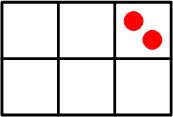
\includegraphics[scale=0.5]{figures/S_T.png}
  \vspace{-0.2cm}
  \caption{Spatial distribution for two tasks}
\end{figure}

\begin{figure}[t]
    \centering
    \subfigure[Distribution 1]{
        \label{fig:S_W1}
        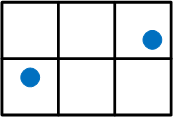
\includegraphics[scale=0.5]{figures/S_W1.png} }
    \subfigure[Distribution 2]{
        \label{fig:S_W2}
        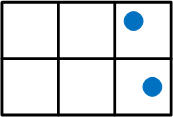
\includegraphics[scale=0.5]{figures/S_W2.png}
    }
    \vspace{-0.2cm}
    \caption{Two spatial distributions for two workers}\label{fig:S_W}
\end{figure}

To account for spatial features of the distribution, in this paper, we use the \textit{Earth Mover's Distance} metric since it has the ability to incorporate the spatial aspect of the distributions when computing their similarity.

\begin{definition}[Earth Mover's Distance]
The Earth Mover's Distance (EMD) is a measure of distance between two probability distributions over a region $D$. If the distributions are interpreted as two different ways of piling up a certain amount of dirt over region $D$, the EMD is the minimum cost of turning one pile into the other; where the cost is assumed to be the amount of dirt moved, times the distance by which it is moved \cite{Rubner98}.
\end{definition}

In order to compute the EMD for two distributions $A$ and $B$, we model it as the  \textit{transportation problem} \cite{Dantzig51}. For each bin $i$, in the distributions, we call cell $i$ a supplier iff $P_A(i) > P_B(i)$ and a consumer iff $P_A(i) < P_B(i)$. If $P_A(i) = P_B(i)$, cell $i$ is neither a supplier nor a consumer. For each supplier $i$, we say $a_i = P_A(i) - P_B(i)$ is the total supply of $i$. Also, the total demand for consumer $j$ is shown as $b_j = P_B(j) - P_A(j)$. Now we can model the problem as a bipartite network flow problem where on one side we have the suppliers and on the other side we have consumer nodes (\cref{fig:MinFlow}). The weight of each edge $c_{ij}$ between supplier $i$ and consumer $j$, is the cost of moving one unit of mass from $i$ to $j$.  Consequently, finding EMD reduces to finding the \textit{Minimum Cost Flow} for this bipartite graph. The Minimum Cost Flow problem can be formalized as the following linear programming problem:\\

\begin{figure}[t]
  \centering
  \label{fig:MinFlow}
  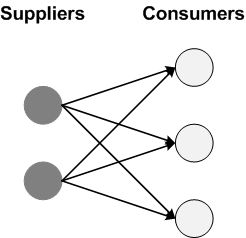
\includegraphics[scale=0.5]{figures/MinFlow.png}
  \vspace{-0.2cm}
  \caption{Example of MinFlow problem with two suppliers and three consumers}
\end{figure}

\setcounter{equation}{0}
\begin{alignat}{2}
\mathbf{minimize}&\mathrlap{\sum_{i \in \mathcal{I}} \sum_{j \in \mathcal{J}} c_{ij}.f_{ij}} \notag\\
\mathbf{subject\ to:}&\phantom{{a}={a}} f_{ij} && \geq 0 \ \quad\quad i \in \mathcal{I}, j \in \mathcal{J}\\
&\phantom{{a}}\sum_{i \in \mathcal{I}} f_{ij} &&= b_j \quad\quad j \in \mathcal{J}\\
&\phantom{{a}}\sum_{j \in \mathcal{J}} f_{ij} &&\leq a_i \quad\quad i \in \mathcal{I}
\end{alignat}

More generally, for any graph $G = (V, E)$ we can assign an integer $b(i)$ to each node in the graph, which indicates the supply (or demand) of the node if $b(i) > 0$ (or $b(i) < 0$) . Then we can rewrite the linear programming problem as: 

\setcounter{equation}{0}
\begin{alignat}{2}
\mathbf{minimize}&\mathrlap{\sum_{(i,j) \in \mathcal{E}} c_{ij}.f_{ij}} \notag\\
\mathbf{subject\ to:}&\phantom{{a}={a}{a}={a}{a}={a}{a}} f_{ij} && \geq 0 \ \quad\quad (i,j) \in \mathcal{E}\\
&\sum_{j:(j,i) \in \mathcal{E}} f_{ij} - \sum_{j:(i,j) \in \mathcal{E}} &&= b(i) \quad\quad i \in \mathcal{V}
\end{alignat}

We use a variation of the algorithm proposed in \cite{Edmonds72}. The solution in \cite{Edmonds72} is based on solving the dual of the linear programming problem:

\setcounter{equation}{0}
\begin{alignat}{2}
\mathbf{maximize}&\quad\mathrlap{\sum_{i \in \mathcal{V}} b(i).\pi(i)} \notag\\
\mathbf{subject\ to:}&\quad\pi(i) - \pi(j) \leq c_{ij} \quad\quad (i,j) \in \mathcal{E}
\end{alignat}

\begin{algorithm}[t]
\caption{MinFlow($V, E, b$)}
\label{algo:MinFlow}
\begin{algorithmic}[1]
\REQUIRE $V$ is the set of nodes, $E$ the set of edges and $b$ the supply/demand of each node
\ENSURE $f$ as the amount of flow on each edge
\STATE for $i \in V$ set $f_i = 0, \pi_i =0$ and $e_i = b_i$
\STATE $U = \max_{i \in V} \left\lbrace\vert b_i\vert \right\rbrace$
\STATE $\delta = 2^{ \lceil \log U \rceil }$
\WHILE {$\delta \geq 1$}
   \STATE $S_{\delta} = \left\lbrace i : e_i \geq \delta \right\rbrace$
   \STATE $C_{\delta} = \left\lbrace i : e_i \leq -\delta \right\rbrace$
   \WHILE{$S_{\delta} \neq \emptyset$ and $C_{\delta} \neq \emptyset$}
     \STATE choose some $s \in S_{\delta}$
     \STATE compute shortest path distances $d_i$ from node $k$ to all other nodes
     \STATE for $i \in V$ set $\pi_i = \pi_i - d_i$
     \STATE choose $c \in C_{\delta}$ such that a path exists from $s$ to $c$
     \STATE augment $\delta$ units of flow along the shortest path from $s$ to $c$
     \STATE update $f, e, S_{\delta}$ and $C_{\delta}$
   \ENDWHILE
   \STATE $\delta = \frac{\delta}{2}$ 
\ENDWHILE
\RETURN $f$
\end{algorithmic}
\end{algorithm}

\cref{algo:MinFlow} is based on the ideas proposed in \cite{Edmonds72}. In line 9, we use Dijkstra's algorithm to compute shortest paths from node $s$ to all other nodes. Instead of using the normal cost of each edge, $c_{ij}$, in computing the shortest paths, \cref{algo:MinFlow} uses a modified cost, $c_{ij}^{*} = c_{ij} - \pi_i + \pi_j$, as the cost of each edge in line 9. It is shown in \cite{Edmonds72} that \cref{algo:MinFlow} runs in polynomial time.